\documentclass{AMdocumentation}
\usepackage{AMfont}
\title{How to compile the dtx files}
\author{Romain Pennec}

\graphicspath{{images/}}

\begin{document}

\OLDmaketitle

\tableofcontents

\vskip1.7cm

\section{Documentation \TeX{} file (dtx)}

Both the documentation and the code of the packages are included in the respective documented source (\extension{.dtx}) files.
Use \cmdbox{pdflatex file.dtx} to extract the documentation (\extension{.pdf}) file.
Use \cmdbox{tex file.dtx} to extract the package (\extension{.sty}) file.
You can use the script \FileName{setup.sh} with the argument \cmdarg{extract}, followed by \cmdarg{doc}, \cmdarg{sty} or \cmdarg{all}. Note that it will run the extraction for \emph{all} the \extension{dtx} files. I will also generate the index and the bibliography, if any. Hence it can takes a while, especially on the network.


\section{\TeXstudio}

\subsection{Installation}

First: use a latex editor that supports \extension{dtx} highlighting! This feature is implemented natively in \TeXstudio [recommanded]. Note: It is also possible to set up \extension{dtx} highlighting TeXworks and Emacs.

\bigskip
\TeXstudio can be downloaded on sourceforge at the address \url{http://texstudio.sourceforge.net/}. 
If you use Ubuntu or similar you can download it from the official ATP repository \emph{but} only the older version \verb|2.6.2| is currently available (today's version is \verb!2.9.4!), therefore I strongly recommend that you get \TeXstudio from its website as the Windows and Mac OS users. If you do not know your Linux distribution enter \cmdbox{lsb_release -d} in a terminal.
\subsection{Configuration}

I will explain how to configurate \TeXstudio to have a convenient way to do this.
If you press F1 (short-key for Build \& View) in order to compile the documentation from \FileName{example.dtx}  you will get an error because by default \TeXstudio looks for the file \FileName{example.tex} (and of course does not find it). In addition we would like to execute \cmdbox*{latex} on the \extension{ins} file to generate the package file \FileName{myfile.sty} from \FileName{example.dtx}.

\begin{itemize}
\item Options $\to$ Configure \TeXstudio 
\item Allow the Advanced Options, if it is not already the case
\item Inside Tab Build, add User Commands: 
	\begin{itemize}
	\item[] \verb!tex %.dtx!
	\item[] \verb!pdflatex -synctex=1 -interaction=nonstopmode %.dtx | txs:///view!
	\end{itemize}
\end{itemize}	


You have also the possibility to use my personal settings for \TeXstudio by loading
the file\footnote{under Options $\to$ Load Profile...}
\begin{center}
\todo{ \FileName{amconfig.txsprofile} }
\end{center}

\begin{itemize}
\item To extract the package or the class: \Alt+\Shift+\keystroke{F1}
\item To compile the documentation: \Alt+\Shift+\keystroke{F2}
\end{itemize}




\section{Pygmentize}

You will also need to install pygmentize, which is required by the package \PackageName{minted}.

\subsection{Installation on Linux}
\begin{itemize}
\item If you have the root privilege, simply enter: \cmdbox[\#>]{sudo apt-get install python-pygments}
\item If not, you will have to download it from the Python Package Index (\url{https://pypi.python.org/pypi/Pygments}), 
extract the archive, go in the directory \verb|Pygments-*| and run
\begin{bashshell}
python setup.py install --prefix=$HOME/local/bin
\end{bashshell}

see details on \url{https://pypi.python.org/pypi/setuptools}

You will have to make sure that the directory \DirPath{\$HOME/local/bin} is included in the \EnvVariable{PATH} variable.

If it is not the case, add the following line at the end of the \FileName{.profile} file
\begin{center}
\verb|export PATH=$PATH:$HOME/local/bin|
\end{center}
You may have to log in again. 

\end{itemize}

\subsection{Installation on Windows}

For explaination on how to install it on Windows: \url{http://pygments.org/download/}

\subsection{Installation on OS X}

Enter \cmdbox[\#>]{sudo easy_install pygments} in the command line.

\section{Up-to-date \LaTeX{} distribution}

The package \PackageName{tcolorbox} is copiously used to typeset the documentation, and
a recent version of  is required (at least version 3.6).
You will also probably need to update the \texlive or \miktex distribution. 

Same goes for the macro package \PackageName{pgf} (available online at \url{https://www.ctan.org/pkg/pgf})
and many other packages or classes.

\subsection{\texlive}

\subsubsection{Upgrade \texlive}

The command \cmdbox{tex --version | head -1} will return your current \texlive version. For example I get on my computer the answer \verb|TeX 3.14159265 (TeX Live 2015)|. With Ubuntu 14.04 LTS you should have \texlive 2013 installed\footnote{According to \url{https://www.tug.org/texlive/debian.html}}, which is fine too. If your distribution is older (for example if you have \texlive 2009) it will be necessary to upgrade it and the least we can say is that it is not a peace of cake. However the following commands should do the work\footnote{Mote details here \url{http://www.tug.org/texlive/doc/texlive-en/texlive-en.html}}:

\begin{bashshell}[title={Bash script to install texlive 2015 on Ubuntu}]
cd ~/Downloads
wget http://ftp.uni-erlangen.de/ctan/systems/texlive/tlnet/install-tl-unx.tar.gz
tar -zxvf install-tl-unx.tar.gz
cd install-tl*
sudo perl install-tl
(*@ {\normalfont\normalcolor you will have to enter \texttt{I}, then it will take a while} @*)
echo "export PATH=\"/usr/local/texlive/2015/bin/x86_64-linux:\$PATH\"" > pathTexLive.sh
chmod +x pathTexLive.sh
sudo mv pathTexLive.sh /etc/profile.d
source /etc/profile.d/pathTexLive.sh
sudo update-texmf
sudo texhash
sudo mktexlsr
tex --version
\end{bashshell}

\subsubsection{Update packages}

\texlive comes with a manager called \cmdbox*{tlmgr} that can be used to update the packages of your distribution\footnote{\url{ http://tex.stackexchange.com/questions/55437/how-do-i-update-my-tex-distribution}}. 

\begin{hint}
Make sure the decompression tool \cmdbox*{xzdec} is installed: \cmdbox[\#>]{apt-get install xzdec}
\end{hint}

\begin{hint}
If you get the message \verb|cannot setup TLPDB|, enter
\cmdbox[\#>]{tlmgr init-usertree}
\end{hint}

\subsection{\miktex}

\todo{ how to update \miktex }

\begin{figure}[h!]
\centering
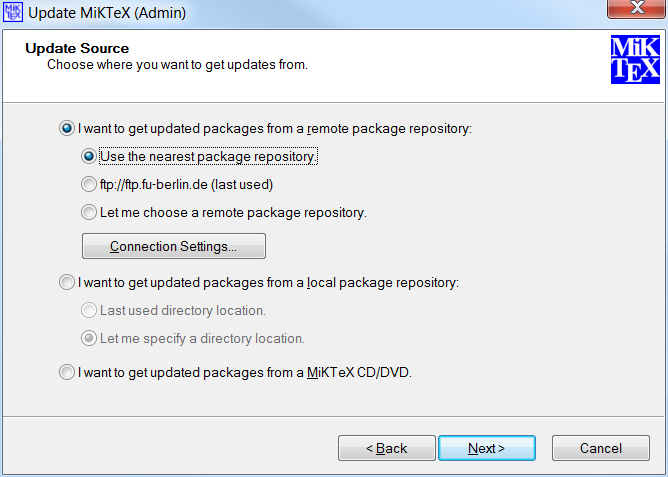
\includegraphics[width=0.75\textwidth]{Update-MiKTeX-1}
\vskip3mm

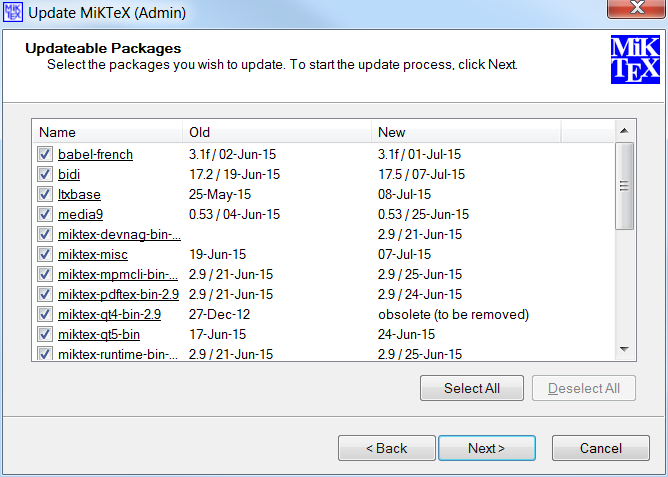
\includegraphics[width=0.75\textwidth]{Update-MiKTeX-2}
\end{figure}

\subsection{\mactex}

Open the \verb!TeX Live Utility! and click on \emph{Actions} $\to$ \emph{Update All Packages}.

\end{document}

Choisir Action I (grand i, Il y en a pour un petit moment)









